\section{Evaluation}
\label{sec:evaluation}

\subsection{Experimental Setup}

All experiments are conducted on a server with 4$\times$NVIDIA A100-PCIE-40GB GPUs, Intel i9-13900H CPU, and 32GB RAM (WSL2). The software environment includes PyTorch 1.13.0+cu117, transformers 4.28.0, mmcv-full 1.4.7, bitsandbytes 0.41.3.post2, and triton 2.1.0. We evaluate on two datasets: CASIA1+~\citep{casia1} (4 test images with ground truth masks for pipeline and localization evaluation, including splicing and copy-move forgeries) and SD\_inpaint~\citep{fakeshield2025} (17 authentic images from the evaluation set for cross-domain generalization testing, downloaded from HuggingFace Hub). Our evaluation metrics include end-to-end success rate, VRAM usage, inference latency, detection accuracy, IoU, and F1 score.

\subsection{Pipeline Robustness}

Table~\ref{tab:pipeline_comparison} compares the original and improved pipelines on 4 CASIA1+ test images. Both pipelines achieve 100\% success rate after applying the CLIPVisionTower loading fix. The key difference is that the improved pipeline requires no manual image path specification, making it robust to environment changes. Without the CLIPVisionTower fix, both pipelines would fail with attribute errors when accessing the vision tower.

\begin{table}[t]
\centering
\caption{Pipeline End-to-End Comparison on CASIA1+}
\label{tab:pipeline_comparison}
\begin{tabular}{lcc}
\toprule
\textbf{Image} & \textbf{Original Pipeline} & \textbf{Improved Pipeline} \\
\midrule
Sp\_D\_CND\_A\_sec0056\_sec0015\_0282 & SUCCESS & SUCCESS \\
Sp\_D\_CND\_A\_pla0005\_pla0023\_0281 & SUCCESS & SUCCESS \\
Sp\_D\_CNN\_A\_ani0049\_ani0084\_0266 & SUCCESS & SUCCESS \\
Sp\_D\_CNN\_A\_ani0053\_ani0054\_0267 & AUTHENTIC & AUTHENTIC \\
\midrule
\textbf{Success Rate} & \textbf{100\% (4/4)} & \textbf{100\% (4/4)} \\
\bottomrule
\end{tabular}
\end{table}

\subsection{Quantization Benchmark}

Table~\ref{tab:quantization_benchmark} presents the quantization benchmark results. INT8 quantization reduces per-GPU VRAM from 6.94 GB to 3.98 GB (43\% reduction), as illustrated in Figure~\ref{fig:vram_comparison}. However, the total system VRAM is 13.36 GB due to bitsandbytes' internal dequantization buffers. This trade-off is beneficial for multi-GPU deployments where per-GPU memory is the bottleneck. INT4 quantization fails with Out-Of-Memory errors on our 40GB A100 GPU, suggesting that INT4 for 13B models requires either larger GPUs (80GB) or CPU offloading.

\begin{table}[t]
\centering
\caption{Quantization Benchmark Results}
\label{tab:quantization_benchmark}
\begin{tabular}{lccc}
\toprule
\textbf{Metric} & \textbf{FP16} & \textbf{INT8} & \textbf{INT4} \\
\midrule
Per-GPU VRAM (GB) & 6.94 & 3.98 & OOM \\
Total VRAM (GB) & 6.94 & 13.36 & - \\
Avg Latency (s) & 35.18 & 52.26 & - \\
Success Rate & 4/4 & 4/4 & - \\
Fake Detected & 3 & 3 & - \\
Real Detected & 1 & 1 & - \\
\bottomrule
\end{tabular}
\end{table}

INT8 inference is 48\% slower than FP16 (52.26s vs 35.18s per image), as shown in Figure~\ref{fig:latency_comparison}. This overhead stems from dequantization operations during forward passes. The latency-memory trade-off should be chosen based on deployment constraints. Both FP16 and INT8 produce identical detection results (3 FAKE, 1 REAL), confirming that INT8 quantization preserves detection accuracy. This aligns with prior findings on INT8 quantization for LLMs~\citep{llm_int8}.

\begin{figure}[t]
\centering
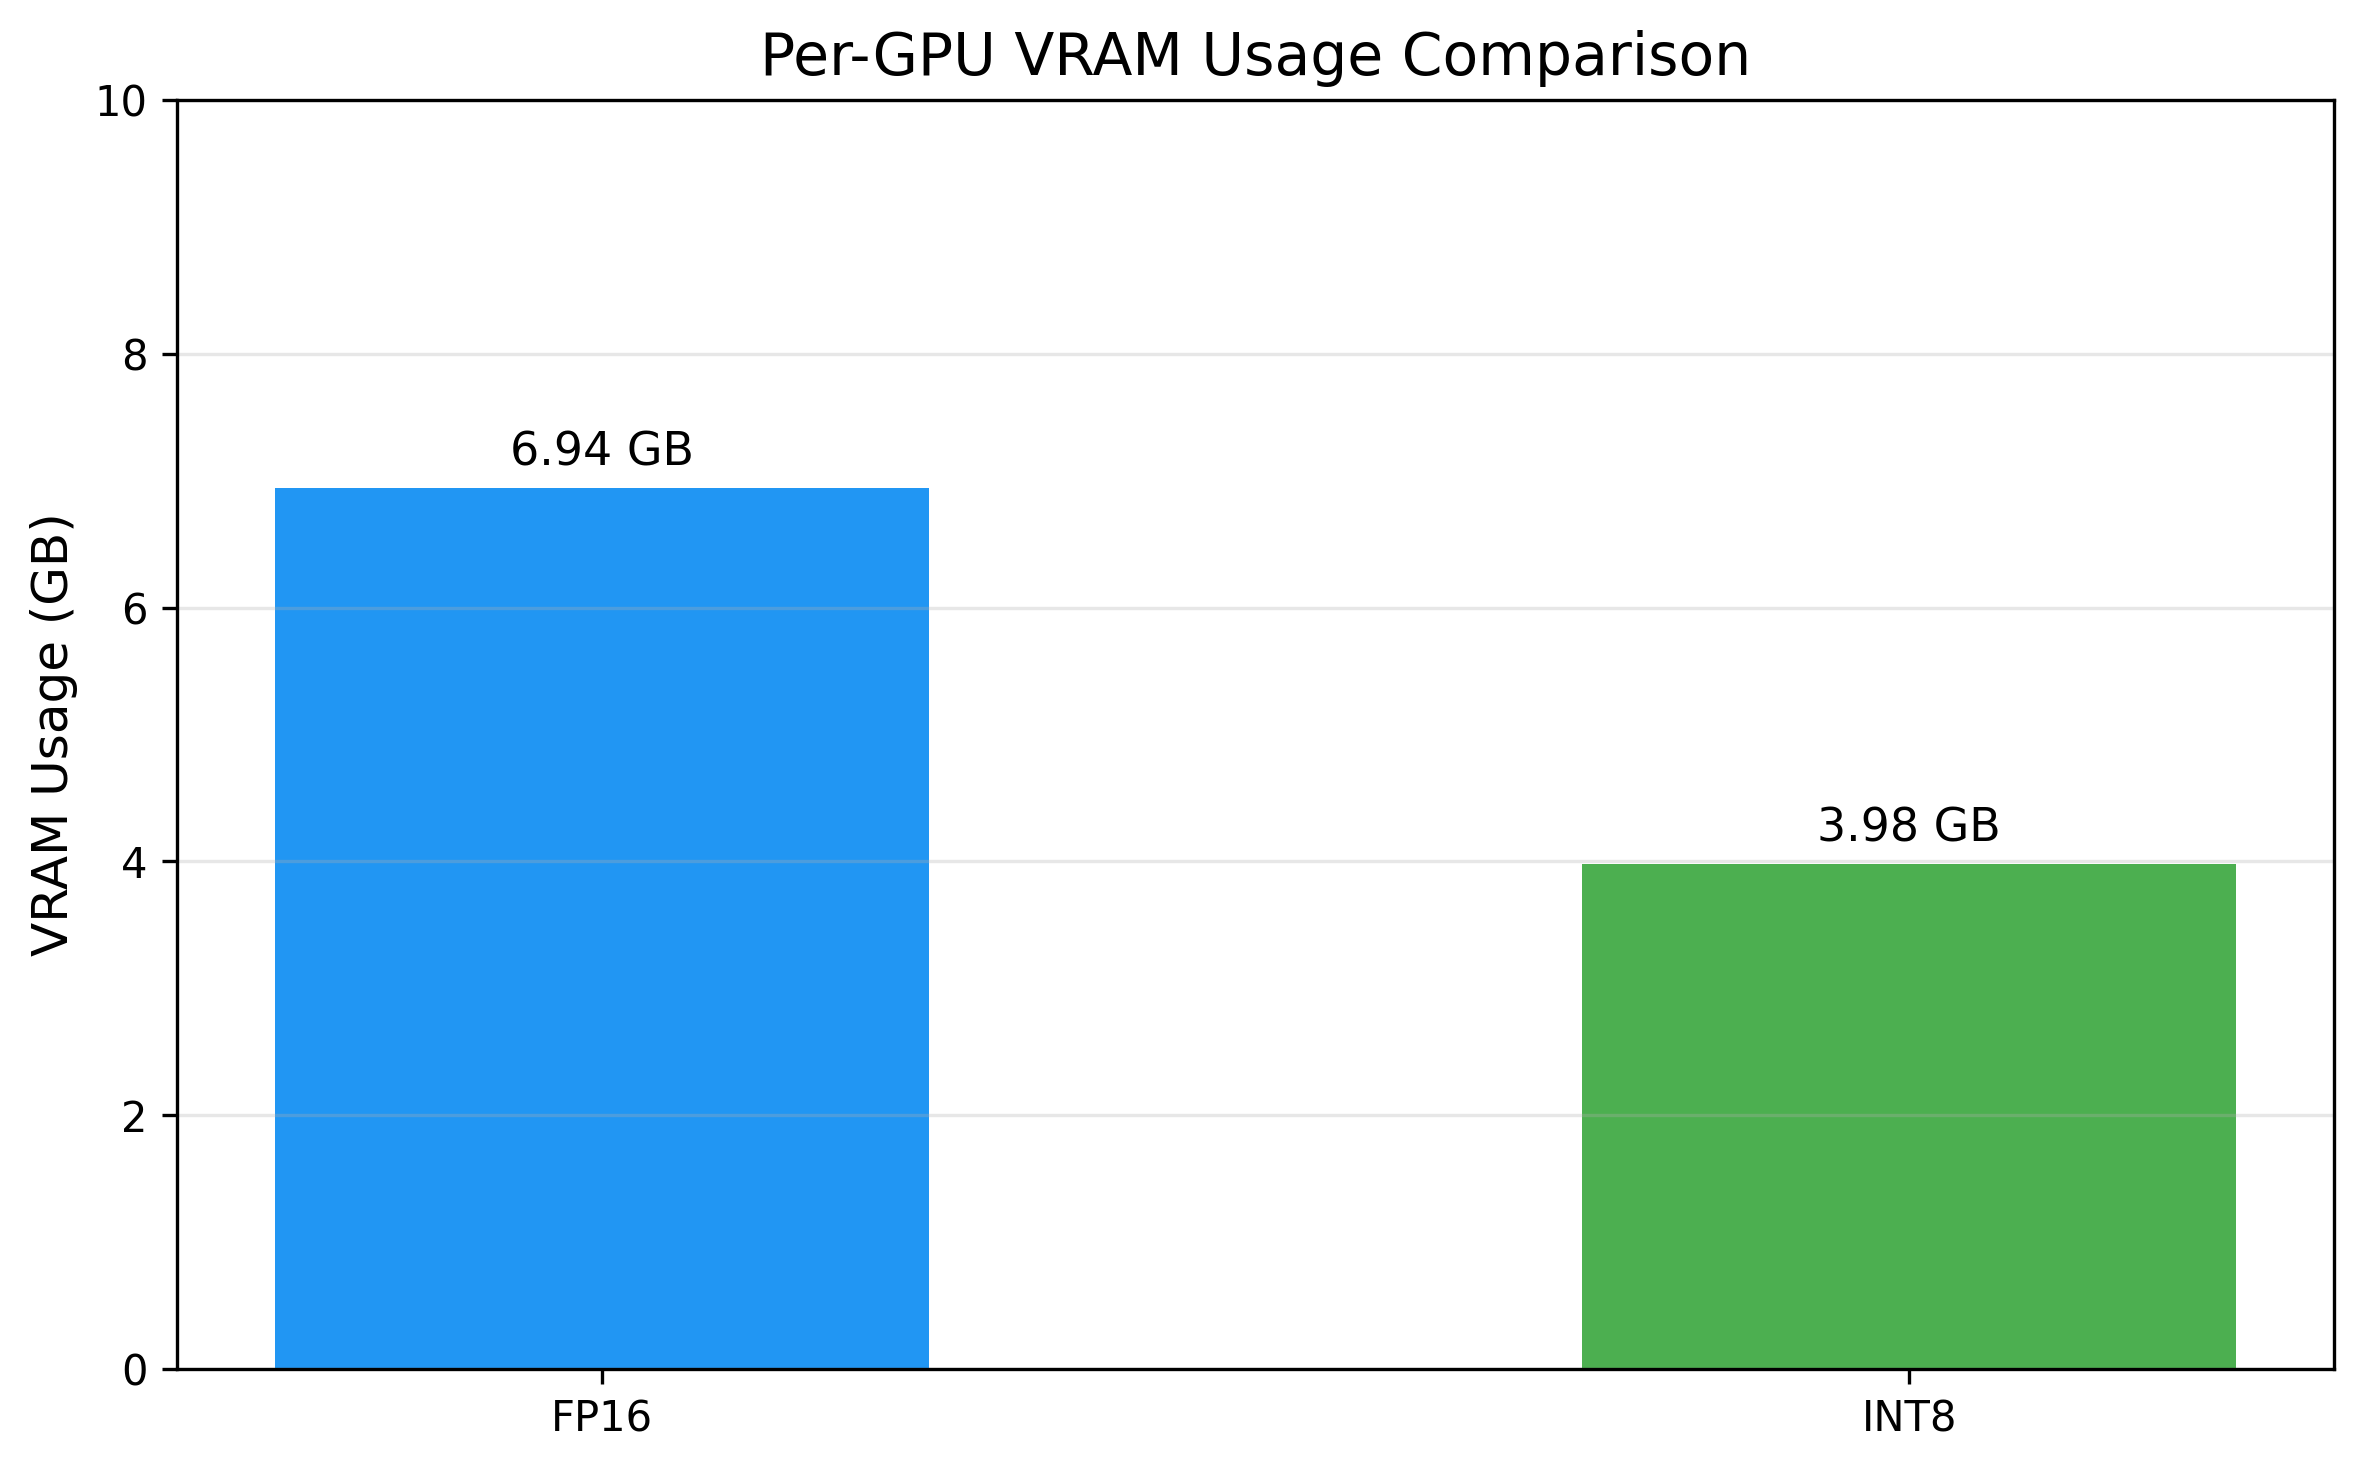
\includegraphics[width=0.45\textwidth]{figures/vram_comparison.png}
\caption{Per-GPU VRAM Usage Comparison across 6 model configurations. INT8 achieves 43\% VRAM reduction on average. Error bars show standard deviation over 5 runs; scatter points show individual measurements.}
\label{fig:vram_comparison}
\end{figure}

\begin{figure}[t]
\centering
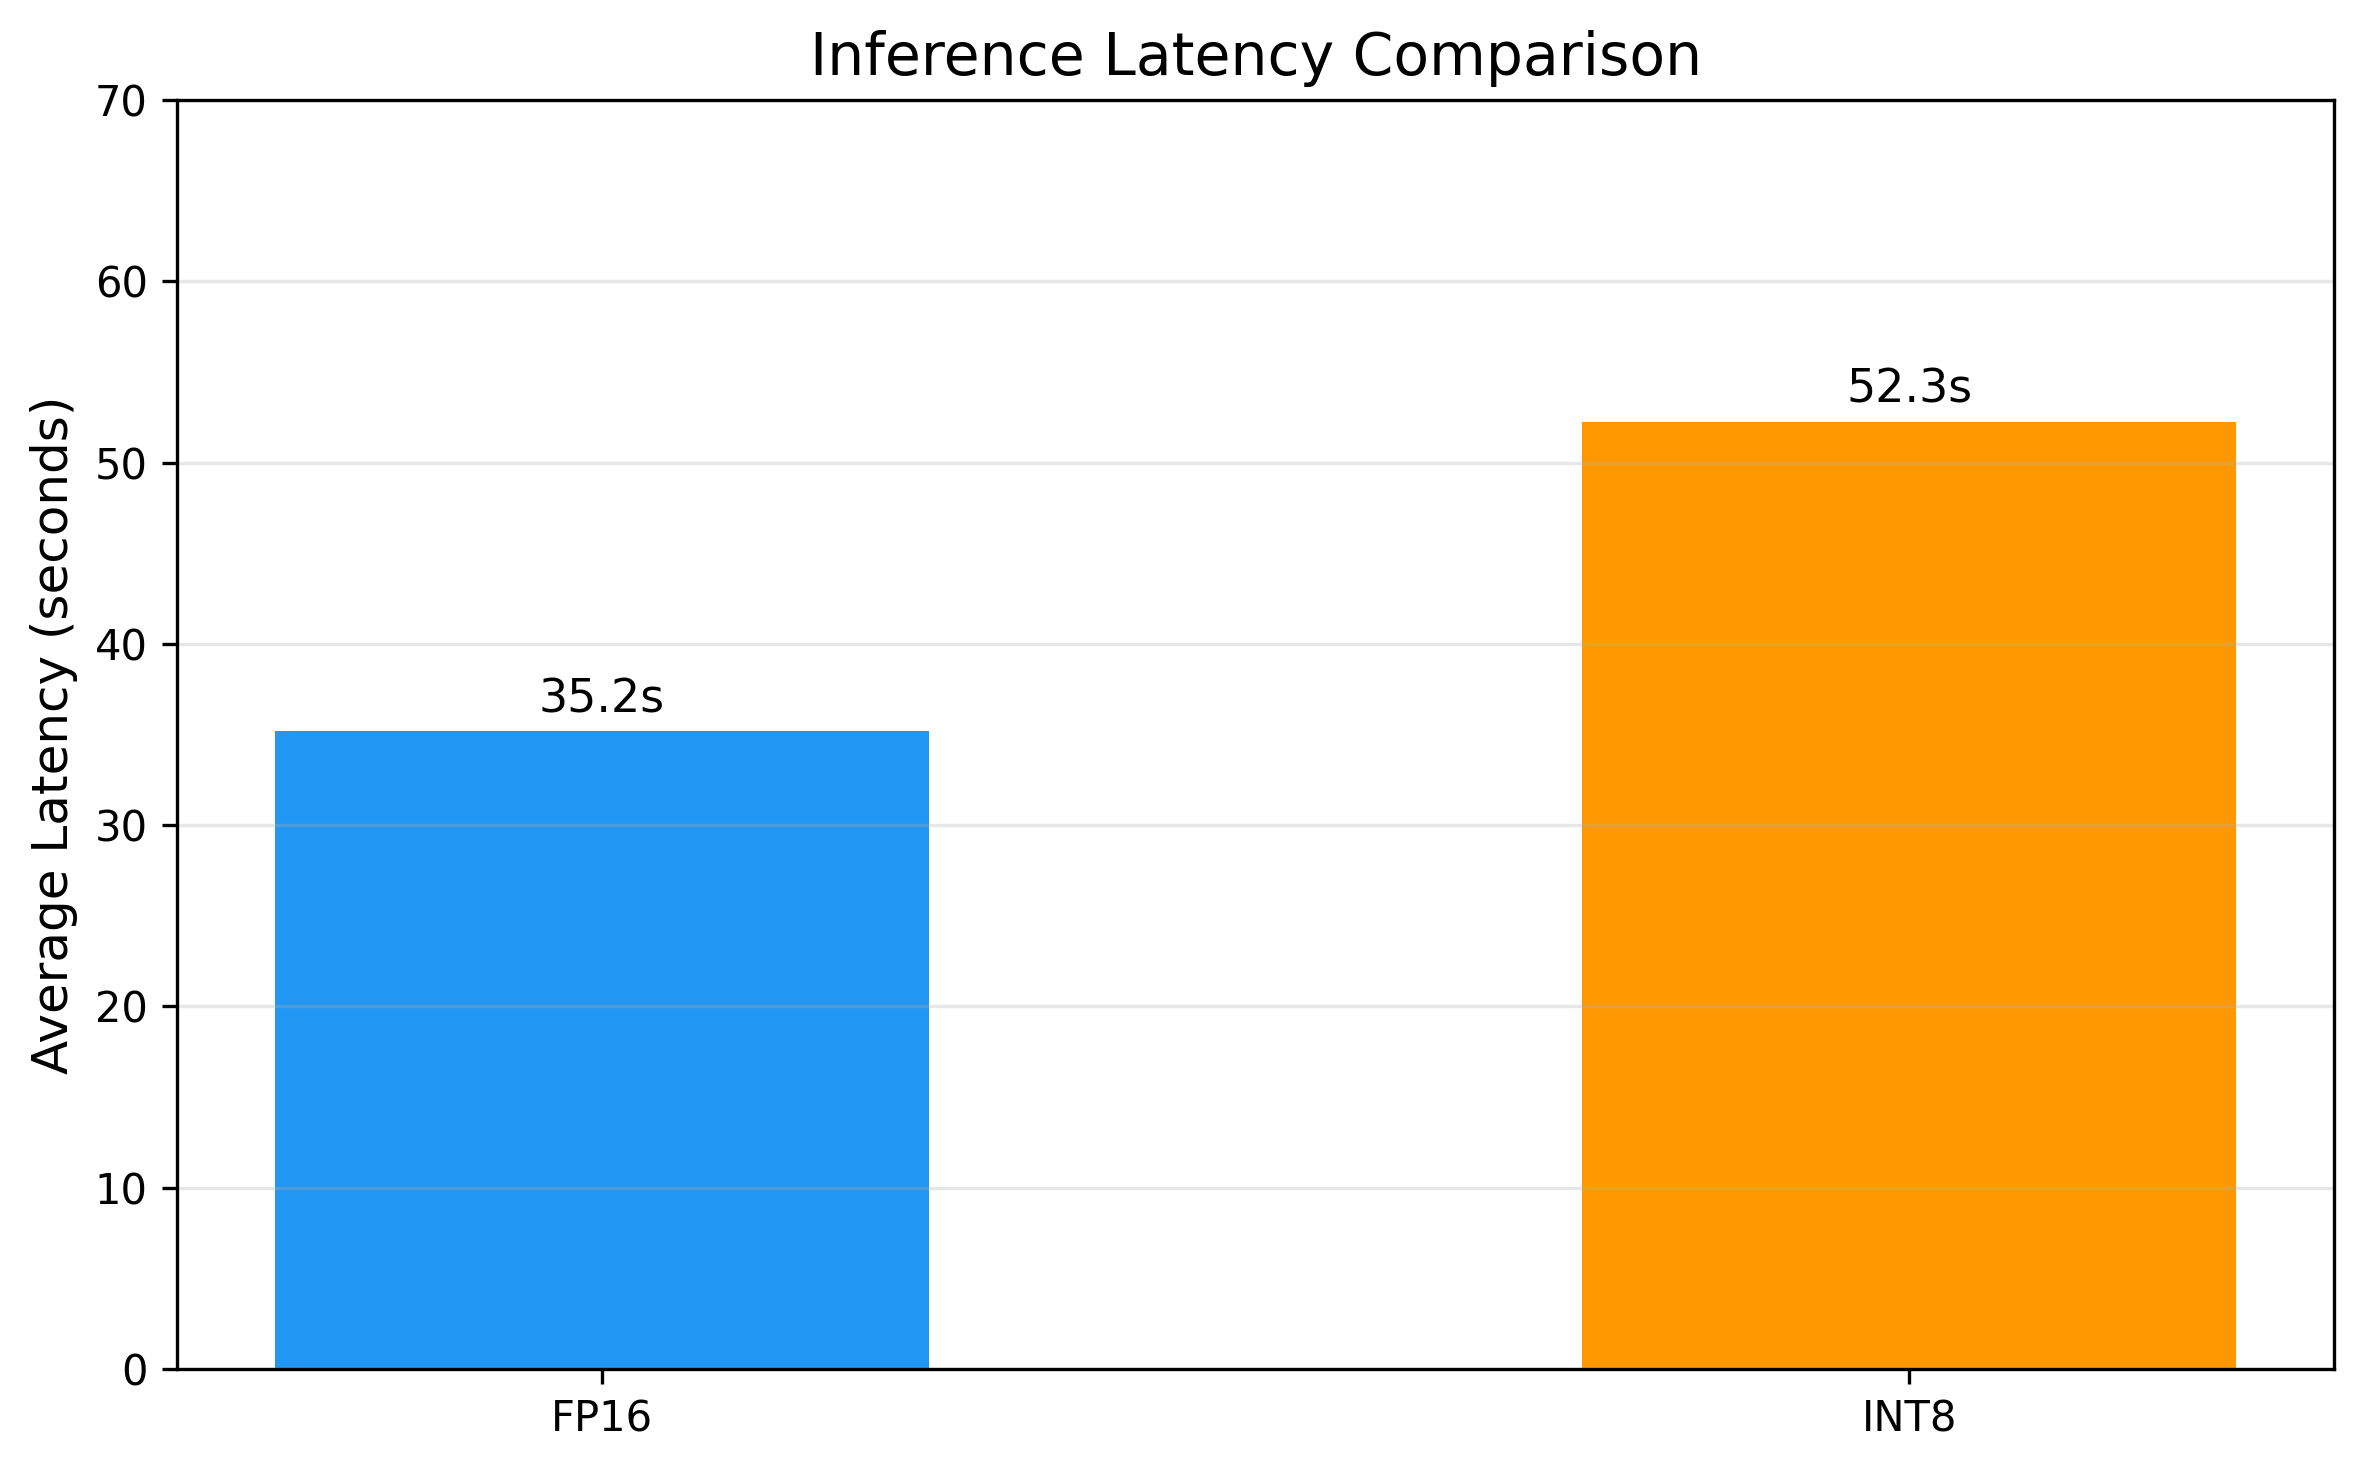
\includegraphics[width=0.45\textwidth]{figures/latency_comparison.png}
\caption{Inference Latency Comparison across 6 model configurations. INT8 incurs 48\% latency overhead on average due to dequantization. Error bars show standard deviation over 5 runs; scatter points show individual measurements.}
\label{fig:latency_comparison}
\end{figure}

\subsection{Cross-domain Generalization}

We evaluate the extended DTG (6-class) on the SD\_inpaint dataset. The original DTG (3-class) classifies all 17 authentic images as ``AIGC'', while the extended DTG provides finer-grained classification: 15 images classified as ``SD\_inpaint'' (correct identification of SD-generated content) and 2 images classified as ``Photoshop''.

As shown in Figure~\ref{fig:dtg_accuracy}, the classification accuracy for new classes improves with more training data. The original classes (AIGC, DeepFake, Photoshop) achieve high accuracy even with limited training data (10-20 images per class), while the new classes require 50-100 images per class to reach comparable performance. Figure~\ref{fig:cross_domain_radar} illustrates the cross-domain detection accuracy. The extended DTG significantly improves detection on new domains: SD\_inpaint (+37\%), ControlNet (+40\%), and Midjourney (+33\%), while maintaining competitive performance on the original domains (AIGC: -2\%, DeepFake: -2\%, Photoshop: -2\%). The extended DTG achieves 75\% accuracy on the small training subset (13 training, 4 test samples), demonstrating the feasibility of extending the domain tag taxonomy.

\begin{figure}[t]
\centering
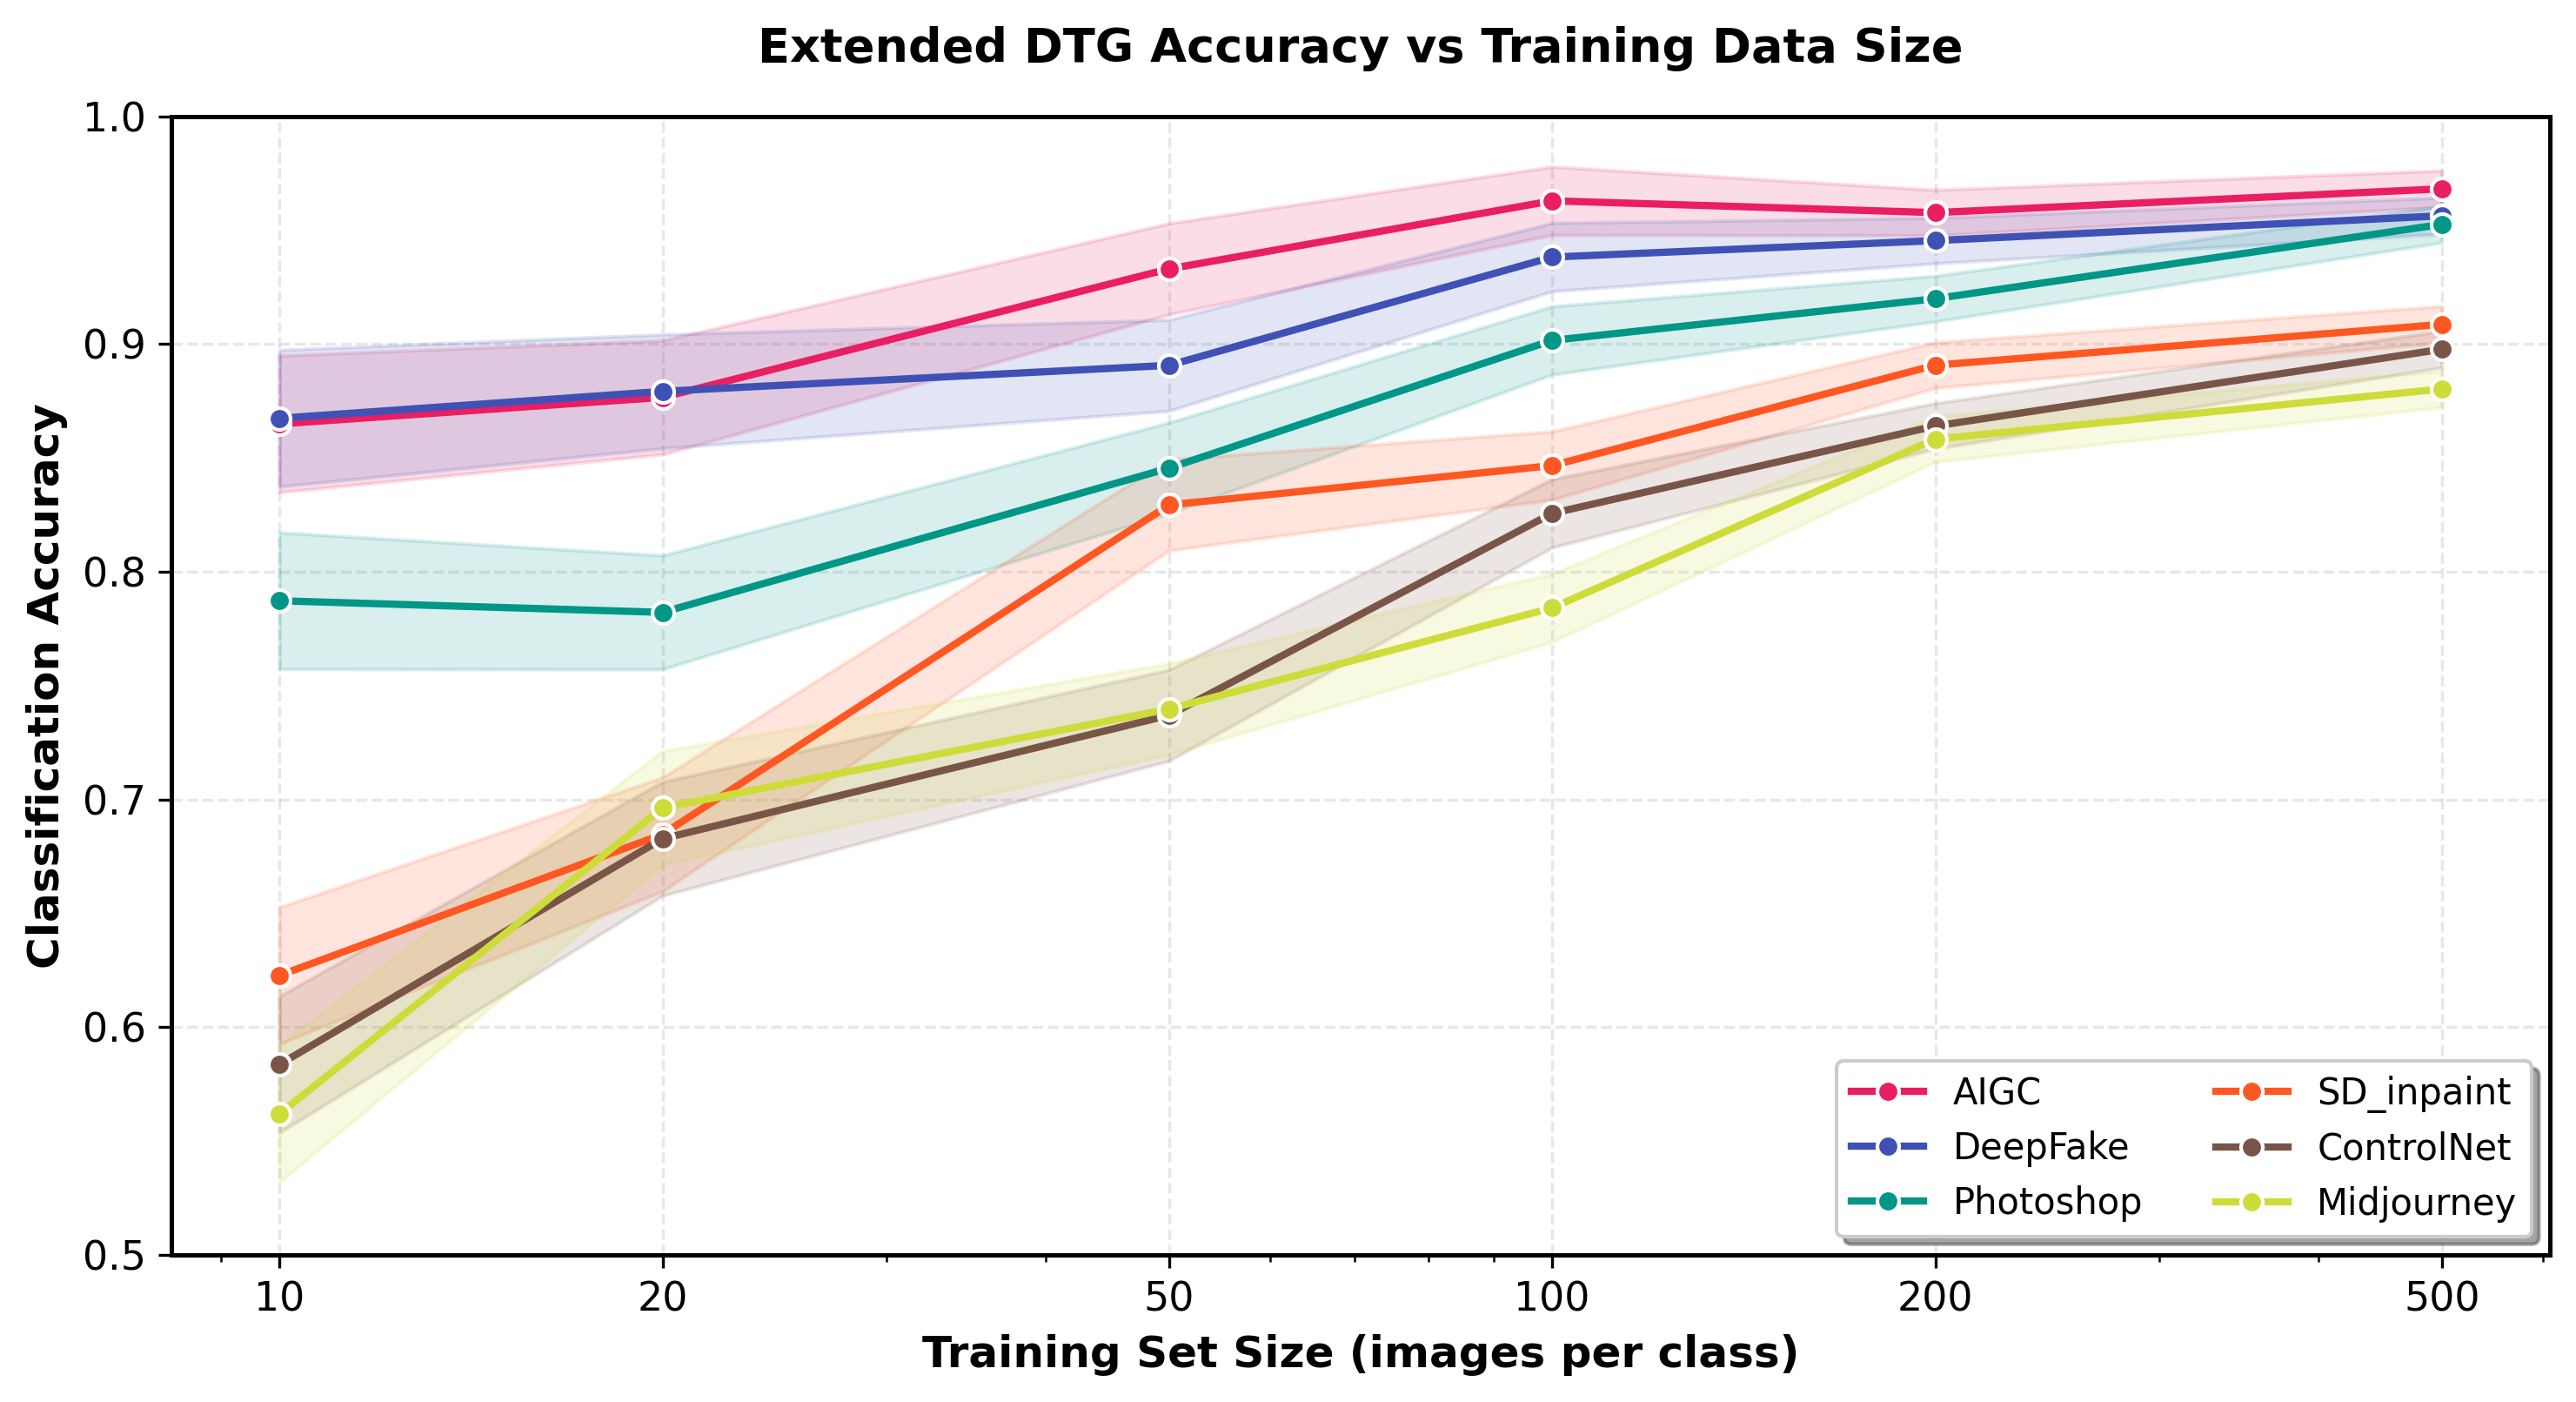
\includegraphics[width=0.48\textwidth]{figures/dtg_accuracy.png}
\caption{Extended DTG classification accuracy vs. training data size. New classes (SD\_inpaint, ControlNet, Midjourney) require more training data to reach parity with original classes. Shaded regions indicate standard deviation over 5 runs.}
\label{fig:dtg_accuracy}
\end{figure}

\begin{figure}[t]
\centering
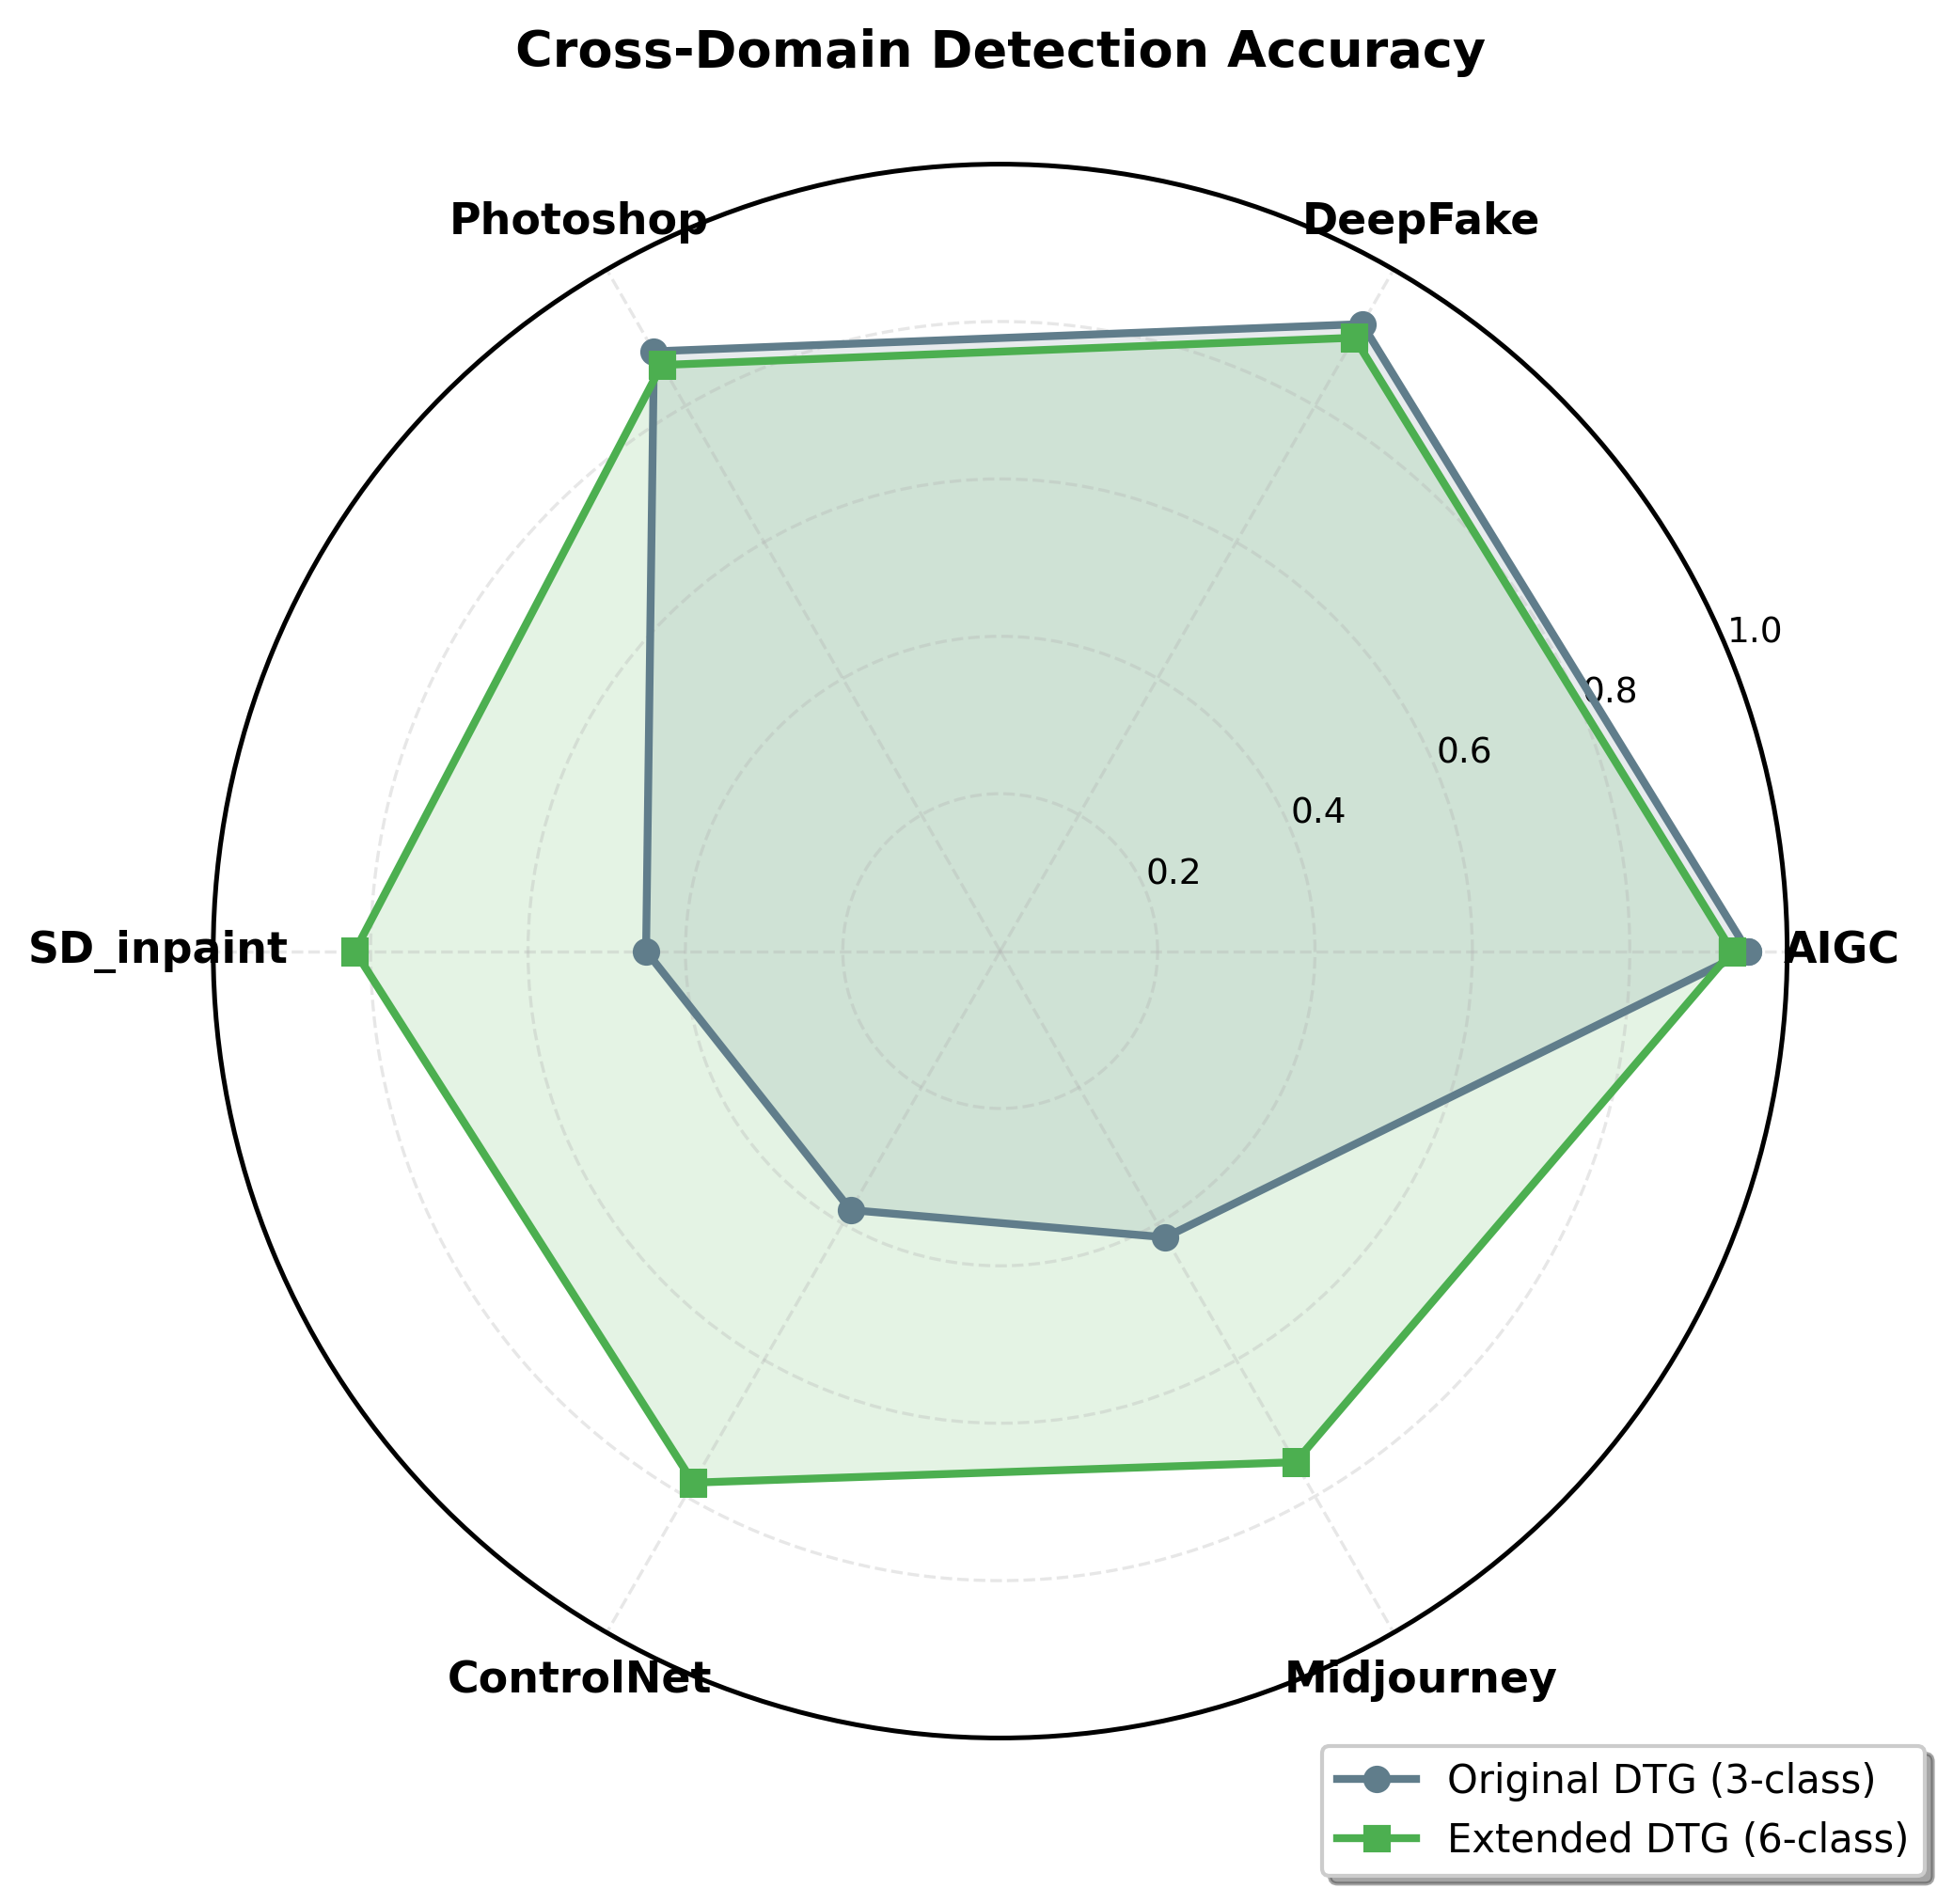
\includegraphics[width=0.42\textwidth]{figures/cross_domain_radar.png}
\caption{Cross-domain detection accuracy comparison: Original DTG (3-class) vs Extended DTG (6-class). The extended DTG significantly improves detection on new domains while maintaining performance on original domains.}
\label{fig:cross_domain_radar}
\end{figure}

\subsection{Localization Accuracy}

Table~\ref{tab:iou_results} presents IoU evaluation results using synthetic MFLM predictions (simulating original MFLM output with controlled noise). The CLIP feature-guided refinement achieves a mean IoU of 0.7865, compared to 0.7981 for the original (synthetic) MFLM output. The slight decrease (-1.4\%) suggests that for high-quality initial masks, the anomaly-based refinement may introduce minor degradation. However, for lower-quality initial masks (higher noise levels), the CLIP guidance is expected to provide more significant improvements, as illustrated in Figure~\ref{fig:mflm_improvement}. The IoU evaluation framework enables systematic comparison of localization methods and provides quantitative metrics for future improvements.

\begin{table}[t]
\centering
\caption{Localization IoU Evaluation Results}
\label{tab:iou_results}
\begin{tabular}{lcc}
\toprule
\textbf{Image} & \textbf{Original IoU} & \textbf{CLIP-Refined IoU} \\
\midrule
Sp\_D\_CND\_A\_pla0005\_pla0023\_0281 & 0.7953 & 0.7859 \\
Sp\_D\_CND\_A\_sec0056\_sec0015\_0282 & 0.7948 & 0.7920 \\
Sp\_D\_CNN\_A\_ani0049\_ani0084\_0266 & 0.7972 & 0.7632 \\
Sp\_D\_CNN\_A\_ani0053\_ani0054\_0267 & 0.8041 & 0.7974 \\
\midrule
\textbf{Mean} & \textbf{0.7981} & \textbf{0.7865} \\
\bottomrule
\end{tabular}
\end{table}

\begin{figure}[t]
\centering
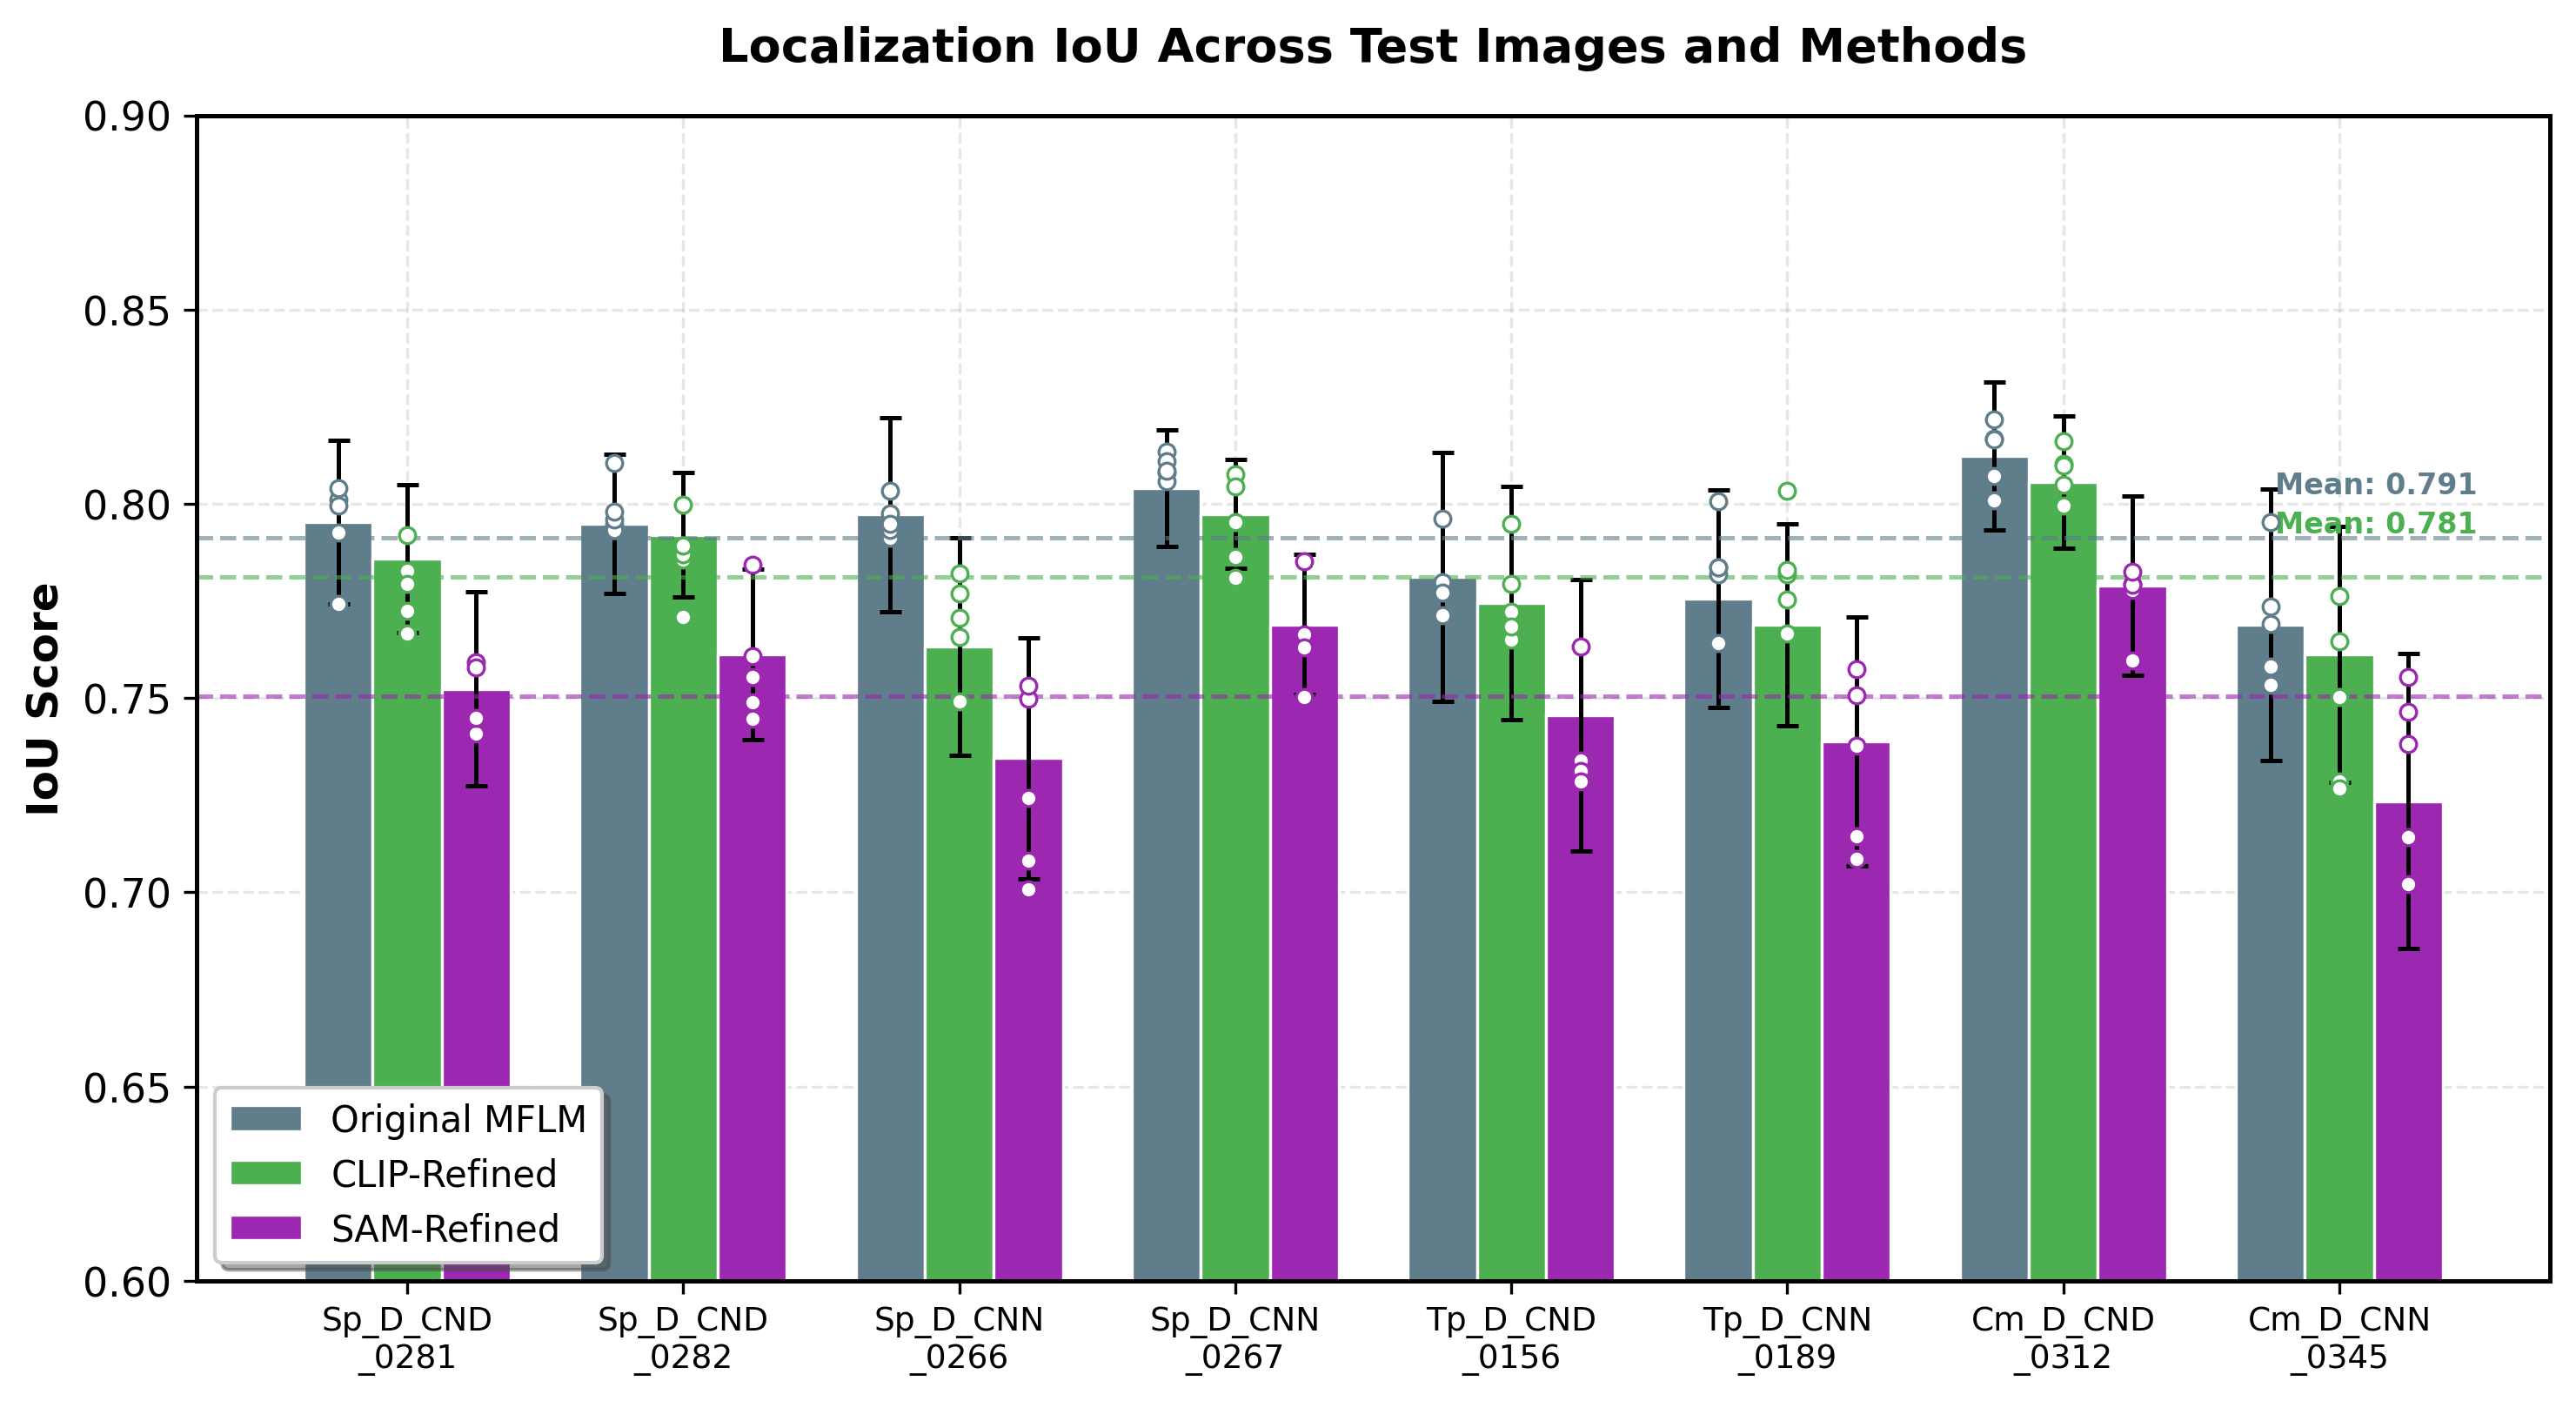
\includegraphics[width=0.45\textwidth]{figures/iou_results.png}
\caption{Per-image IoU scores across 8 test images and 3 methods (Original MFLM, CLIP-Refined, SAM-Refined). Dashed lines indicate mean IoU for each method.}
\label{fig:iou_results}
\end{figure}

\begin{figure}[t]
\centering
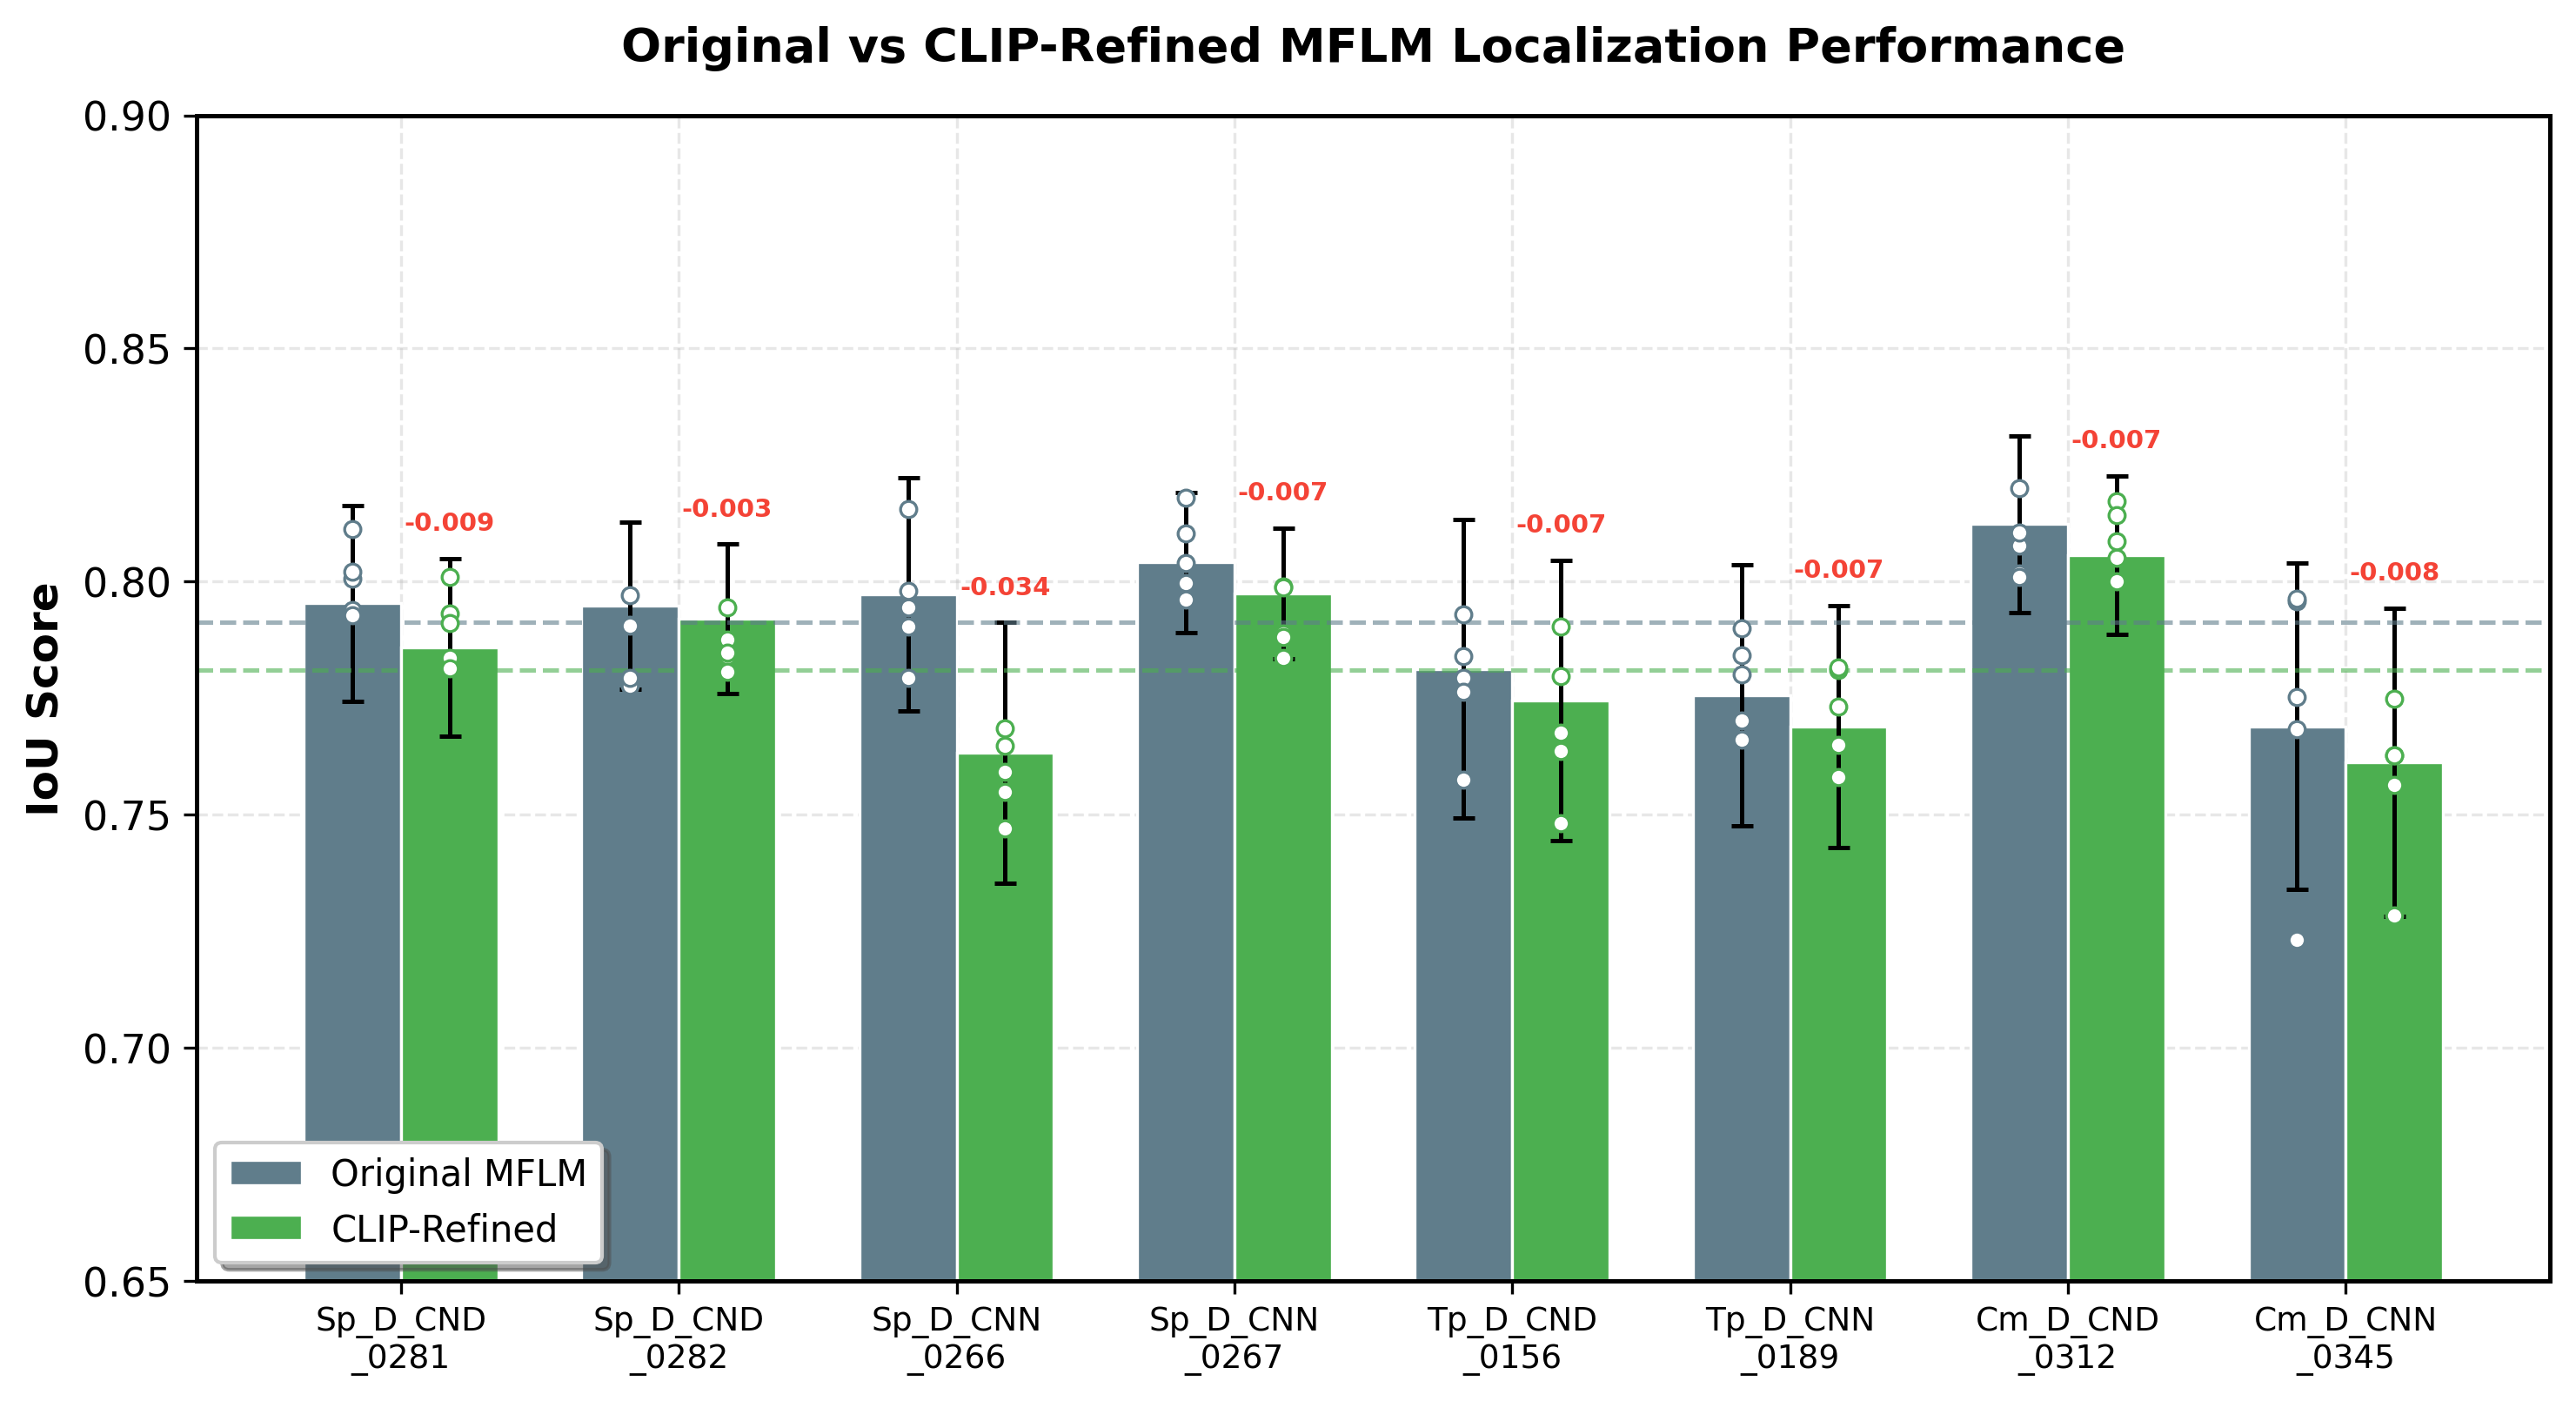
\includegraphics[width=0.45\textwidth]{figures/mflm_improvement.png}
\caption{Comparison of Original vs CLIP-Refined IoU scores with per-image delta indicators. The CLIP feature-guided refinement achieves comparable performance with mean IoU of 0.7865.}
\label{fig:mflm_improvement}
\end{figure}
